\documentclass[aspectratio=169,11pt]{beamer}
\usetheme{Madrid}
\usecolortheme{seahorse}

\usepackage[T1]{fontenc}
\usepackage{lmodern}
\usepackage{booktabs}
\usepackage{array}
\usepackage{xcolor}
\usepackage{listings}
\usepackage{tikz}
\usetikzlibrary{shapes.geometric, arrows.meta, positioning, fit}
\usepackage{multirow}
\usepackage{graphicx}
\graphicspath{{struct_imgs/}}

\definecolor{acceptgreen}{RGB}{34,139,34}
\definecolor{rejectred}{RGB}{178,34,34}
\definecolor{warnblue}{RGB}{0,90,156}
\definecolor{codebg}{RGB}{245,245,245}
\definecolor{phase1}{RGB}{200,220,255}
\definecolor{phase15}{RGB}{185,210,245}
\definecolor{phase2}{RGB}{220,240,200}
\definecolor{phase25}{RGB}{255,235,200}
\definecolor{phase3}{RGB}{240,210,230}
\definecolor{phase4}{RGB}{230,220,250}

\lstset{
  basicstyle=\ttfamily\scriptsize,
  backgroundcolor=\color{codebg},
  frame=single,
  breaklines=true,
  columns=fullflexible,
  keepspaces=true,
}

\setbeamertemplate{navigation symbols}{}
\setbeamerfont{frametitle}{size=\normalsize}
\setbeamerfont{title}{size=\large}

\title{PubChem Cross-Validation for ModelSEED Compounds}
\subtitle{Full-Dataset Validation and Correction Results}
\author{ModelSEED Database Cleanup}
\date{\today}

\begin{document}

% =====================================================================
\begin{frame}
\titlepage
\end{frame}

% =====================================================================
% PART 1: DATASET
% =====================================================================

\begin{frame}{Dataset Overview}

\begin{columns}[T]
\begin{column}{0.42\textwidth}
\begin{table}[h]
\centering
\small
\begin{tabular}{lr}
\toprule
\textbf{Metric} & \textbf{Count} \\
\midrule
Total compounds        & 36,844 \\
With structures        & 30,323 \\
With names             & 45,171 \\
\textbf{Validated}     & \textbf{30,321} \\
\bottomrule
\end{tabular}
\end{table}
\end{column}

\begin{column}{0.54\textwidth}
\textbf{Goal}: Validate whether compound structures in ModelSEED
correctly correspond to their PubChem records, and apply
evidence-based corrections.

\medskip
\textbf{Approach}: Multi-phase pipeline that queries PubChem
using cross-references (ChEBI/KEGG), compound names, and
direct structure lookups (InChIKey/InChI), then classifies
discrepancies and applies validated corrections.

\medskip
\textbf{Scope}: 30,321 compounds with both a searchable
identifier and a stored InChIKey.
\end{column}
\end{columns}

\end{frame}

% =====================================================================
% PART 2: METHODOLOGY
% =====================================================================

\begin{frame}{Methodology: Pipeline Overview}

\vspace{-2pt}
\begin{center}
\resizebox{0.98\textwidth}{!}{%
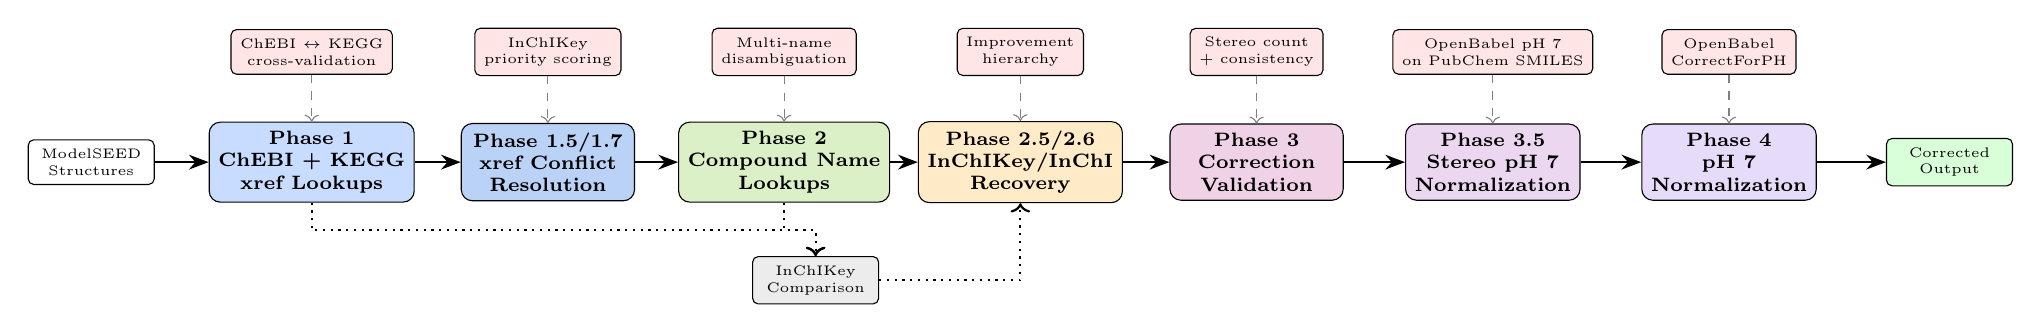
\begin{tikzpicture}[
  every node/.style={font=\scriptsize},
  phase/.style={rectangle, draw, rounded corners=4pt, minimum width=2.2cm,
                minimum height=0.9cm, align=center, font=\scriptsize\bfseries},
  smallbox/.style={rectangle, draw, rounded corners=2pt, minimum width=1.6cm,
                   minimum height=0.5cm, align=center, font=\tiny},
  arr/.style={-{Stealth[length=2.5mm]}, thick},
]
  % Phase boxes
  \node[phase, fill=phase1] (p1) at (0,0)
    {Phase 1\\ChEBI + KEGG\\xref Lookups};
  \node[phase, fill=phase15] (p15) at (3,0)
    {Phase 1.5/1.7\\xref Conflict\\Resolution};
  \node[phase, fill=phase2] (p2) at (6,0)
    {Phase 2\\Compound Name\\Lookups};
  \node[phase, fill=phase25] (p25) at (9,0)
    {Phase 2.5/2.6\\InChIKey/InChI\\Recovery};
  \node[phase, fill=phase3] (p3) at (12,0)
    {Phase 3\\Correction\\Validation};
  \node[phase, fill=phase3!50!phase4] (p35) at (15,0)
    {Phase 3.5\\Stereo pH~7\\Normalization};
  \node[phase, fill=phase4] (p4) at (18,0)
    {Phase 4\\pH~7\\Normalization};

  % Input/output
  \node[smallbox] (input) at (-2.8,0) {ModelSEED\\Structures};
  \node[smallbox, fill=green!15] (output) at (20.8,0) {Corrected\\Output};

  % Classification step
  \node[smallbox, fill=gray!15] (classify) at (6.4,-1.5)
    {InChIKey\\Comparison};

  % Cross-validation annotations
  \node[smallbox, fill=red!10] (xval1) at (0,1.4)
    {ChEBI $\leftrightarrow$ KEGG\\cross-validation};
  \node[smallbox, fill=red!10] (xval15) at (3,1.4)
    {InChIKey\\priority scoring};
  \node[smallbox, fill=red!10] (xval2) at (6,1.4)
    {Multi-name\\disambiguation};
  \node[smallbox, fill=red!10] (xval25) at (9,1.4)
    {Improvement\\hierarchy};
  \node[smallbox, fill=red!10] (xval3) at (12,1.4)
    {Stereo count\\+ consistency};
  \node[smallbox, fill=red!10] (xval35) at (15,1.4)
    {OpenBabel pH~7\\on PubChem SMILES};
  \node[smallbox, fill=red!10] (xval4) at (18,1.4)
    {OpenBabel\\CorrectForPH};

  % Arrows
  \draw[arr] (input) -- (p1);
  \draw[arr] (p1) -- (p15);
  \draw[arr] (p15) -- (p2);
  \draw[arr] (p2) -- (p25);
  \draw[arr] (p25) -- (p3);
  \draw[arr] (p3) -- (p35);
  \draw[arr] (p35) -- (p4);
  \draw[arr] (p4) -- (output);

  % Validation arrows
  \draw[->, dashed, gray] (xval1) -- (p1);
  \draw[->, dashed, gray] (xval15) -- (p15);
  \draw[->, dashed, gray] (xval2) -- (p2);
  \draw[->, dashed, gray] (xval25) -- (p25);
  \draw[->, dashed, gray] (xval3) -- (p3);
  \draw[->, dashed, gray] (xval35) -- (p35);
  \draw[->, dashed, gray] (xval4) -- (p4);

  % Classification arrows
  \draw[->, dotted, thick] (p1.south) -- ++(0,-0.35) -| (classify);
  \draw[->, dotted, thick] (p2.south) -- ++(0,-0.35) -| (classify);
  \draw[->, dotted, thick] (classify) -| (p25.south);
\end{tikzpicture}%
}
\end{center}

\smallskip
\footnotesize
Each phase queries PubChem for the compound's InChIKey, which is compared
block-by-block against the stored InChIKey to classify the result.
Phases~2.5/2.6 recover unresolved compounds via direct structure lookups.
Phase~3.5 normalizes accepted STEREO\_DIFF corrections to pH~7, preventing
PubChem's neutral protonation from overwriting curated ionization states.
Phase~4 normalizes remaining compounds' protonation to pH~7.
All results are cached in SQLite for resumability.

\end{frame}

% =====================================================================
\begin{frame}{Methodology: InChIKey-Based Classification}

\begin{columns}[T]
\begin{column}{0.50\textwidth}

\textbf{InChIKey structure} (three hyphen-separated blocks):

\smallskip
{\ttfamily\small
\underbrace{\texttt{BSYNRYMUTXBXSQ}}_{\text{Connectivity (14)}}%
-\underbrace{\texttt{UHFFFAOYSA}}_{\text{Stereo (10)}}%
-\underbrace{\texttt{N}}_{\text{P}}%
}

\smallskip
{\scriptsize Block~1: connectivity (atoms, bonds).
Block~2: stereo (E/Z, R/S).
Block~3: protonation (N\,=\,neutral).}

\smallskip
\textbf{Classification by block comparison:}

\vspace{-4pt}
\begin{table}[h]
\centering
\footnotesize
\begin{tabular}{lccc}
\toprule
\textbf{Category} & \textbf{Blk 1} & \textbf{Blk 2} & \textbf{Blk 3} \\
\midrule
MATCH            & = & = & = \\
PROTONATION\_DIFF & = & = & $\neq$ \\
STEREO\_DIFF      & = & $\neq$ & --- \\
MISMATCH          & $\neq$ & --- & --- \\
\bottomrule
\end{tabular}
\end{table}

\end{column}

\begin{column}{0.46\textwidth}
\textbf{Interpretation:}\small
\begin{description}\setlength\itemsep{0pt}
  \item[MATCH] Identical molecule.
  \item[PROT.\ DIFF] Same molecule, different protonation
    state. Represents the same compound at different pH.
  \item[STEREO\_DIFF] Same connectivity, different
    stereochemistry. May indicate missing stereocenters.
  \item[MISMATCH] Different molecular graph ---
    incorrect mapping or tautomeric difference.
\end{description}

\smallskip
\footnotesize
Hierarchical comparison (Block~1 first, then~2, then~3)
identifies the most significant differences first.
Only STEREO\_DIFF is eligible for automated correction.
\end{column}
\end{columns}

\end{frame}

% =====================================================================
\begin{frame}{Methodology: PubChem Lookup Strategies (1/2)}
\small
\begin{columns}[T]
\begin{column}{0.48\textwidth}
\textbf{Phase 1: Cross-reference lookups}
\begin{itemize}\setlength\itemsep{0pt}
  \item Query PubChem by ChEBI and KEGG registry IDs
  \item Both identifiers queried when available ---
        conflicting CIDs $\to$ \texttt{XREF\_CONFLICT}
  \item Highest confidence (curated mappings)
\end{itemize}

\smallskip
\textbf{Phase 1.5/1.7: Conflict resolution}
\begin{itemize}\setlength\itemsep{0pt}
  \item Resolve ChEBI$\neq$KEGG conflicts by comparing
        candidate InChIKeys to stored InChIKey
  \item Priority scoring: exact match $>$ block~1+2 $>$ block~1
  \item Remaining conflicts: fetch full CID properties
\end{itemize}
\end{column}

\begin{column}{0.48\textwidth}
\textbf{Phase 2: Name lookups}
\begin{itemize}\setlength\itemsep{0pt}
  \item For compounds without xrefs or failed lookups
  \item Up to 3 names per compound (scored by quality)
  \item Multi-name disambiguation via InChIKey matching
\end{itemize}

\smallskip
\textbf{Phase 2.5: InChIKey recovery}
\begin{itemize}\setlength\itemsep{0pt}
  \item For NOT\_FOUND, MISMATCH, or STEREO\_DIFF
        after Phases 1--2
  \item Query PubChem with the \textbf{stored InChIKey}
  \item 97.0\% match rate --- indicates initial discrepancies
        were due to incorrect mappings, not incorrect structures
\end{itemize}
\end{column}
\end{columns}

\end{frame}

% =====================================================================
\begin{frame}{Methodology: PubChem Lookup Strategies (2/2)}
\small
\begin{columns}[T]
\begin{column}{0.48\textwidth}
\textbf{Phase 2.6: InChI recovery}\footnotesize
\begin{itemize}\setlength\itemsep{0pt}
  \item For still-unresolved compounds after Phase~2.5
  \item Direct InChI lookup in PubChem
\end{itemize}

\small\textbf{Phase 3: Correction validation}\footnotesize
\begin{itemize}\setlength\itemsep{0pt}
  \item Fetch full CID properties for STEREO\_DIFF and MISMATCH
  \item Apply validation gate (stereo counting, consistency)
  \item Cache validated corrections in SQLite
\end{itemize}

\small\textbf{Phase 3.5: Stereo pH~7 normalization}\footnotesize
\begin{itemize}\setlength\itemsep{0pt}
  \item \texttt{CorrectForPH(7.0)} on accepted STEREO\_DIFF SMILES
  \item Prevents PubChem neutral protonation from overwriting
        curated ionization states
\end{itemize}
\end{column}

\begin{column}{0.48\textwidth}
\textbf{Phase 4: pH~7 normalization}\footnotesize
\begin{itemize}\setlength\itemsep{0pt}
  \item OpenBabel \texttt{CorrectForPH(7.0)} on remaining compounds
  \item Only apply if protonation-only change (no connectivity change)
  \item Rejects free phosphate over-deprotonation ($\text{p}K_{\text{a}4}{>}7$)
\end{itemize}

\small\textbf{Improvement hierarchy} (Phase~2.5):\footnotesize
\begin{itemize}\setlength\itemsep{0pt}
  \item NOT\_FOUND $\to$ any result
  \item MISMATCH $\to$ MATCH, PROT\_DIFF, or STEREO\_DIFF
  \item STEREO\_DIFF $\to$ MATCH or PROT\_DIFF
\end{itemize}
\end{column}
\end{columns}

\end{frame}

% =====================================================================
\begin{frame}{Methodology: Correction Validation Gate}

\begin{center}
\resizebox{0.95\textwidth}{!}{%
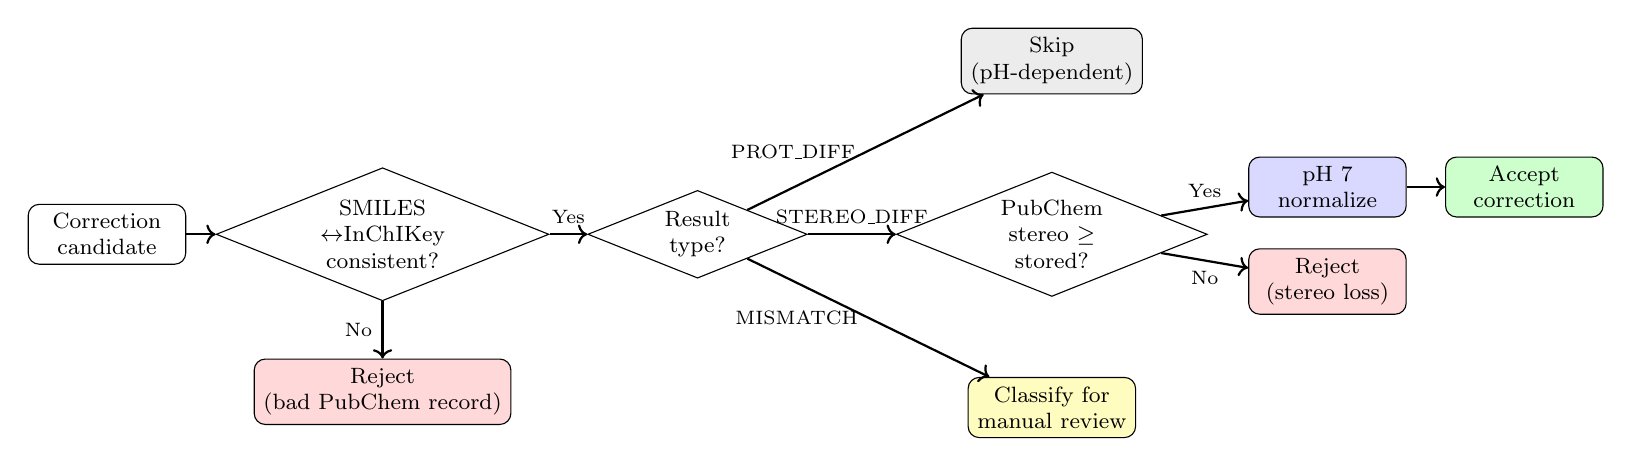
\begin{tikzpicture}[
  every node/.style={font=\footnotesize},
  box/.style={rectangle, draw, rounded corners, minimum width=2cm,
              minimum height=0.6cm, align=center},
  decision/.style={diamond, draw, aspect=2.5, inner sep=2pt,
                   align=center, font=\footnotesize},
  accept/.style={box, fill=green!20},
  reject/.style={box, fill=red!15},
  review/.style={box, fill=yellow!25},
  skip/.style={box, fill=gray!15},
]
  \node[box] (input) at (0,0) {Correction\\candidate};
  \node[decision] (consist) at (3.5,0) {SMILES\\$\leftrightarrow$InChIKey\\consistent?};

  \node[reject] (c_no) at (3.5,-2) {Reject\\(bad PubChem record)};

  \node[decision] (type) at (7.5,0) {Result\\type?};
  \node[skip] (prot) at (12,2.2) {Skip\\(pH-dependent)};
  \node[decision] (stereo) at (12,0) {PubChem\\stereo $\geq$\\stored?};
  \node[review] (mm_review) at (12,-2.2) {Classify for\\manual review};

  \node[box, fill=blue!15] (ph7norm) at (15.5,0.6) {pH~7\\normalize};
  \node[accept] (s_ok) at (18,0.6) {Accept\\correction};
  \node[reject] (s_no) at (15.5,-0.6) {Reject\\(stereo loss)};

  \draw[->,thick] (input) -- (consist);
  \draw[->,thick] (consist) -- node[left,font=\scriptsize]{No} (c_no);
  \draw[->,thick] (consist) -- node[above,font=\scriptsize]{Yes} (type);
  \draw[->,thick] (type) -- node[left,font=\scriptsize]{PROT\_DIFF} (prot);
  \draw[->,thick] (type) -- node[above,font=\scriptsize]{STEREO\_DIFF} (stereo);
  \draw[->,thick] (type) -- node[left,font=\scriptsize]{MISMATCH} (mm_review);
  \draw[->,thick] (stereo) -- node[above,font=\scriptsize]{Yes} (ph7norm);
  \draw[->,thick] (ph7norm) -- (s_ok);
  \draw[->,thick] (stereo) -- node[below,font=\scriptsize]{No} (s_no);
\end{tikzpicture}%
}
\end{center}

\smallskip
\begin{columns}[T]
\begin{column}{0.48\textwidth}
\footnotesize
\textbf{STEREO\_DIFF}: Accepted only if PubChem defines $\geq$ stereocenters
than the stored structure \textit{and} shared stereocenters are not inverted
(InChI stereo layer comparison). Accepted corrections are then normalized
to pH~7 (OpenBabel) to preserve the curated ionization state.
\end{column}
\begin{column}{0.48\textwidth}
\footnotesize
\textbf{MISMATCH sub-classification} (all for manual review):\\
Formula gate $\to$ ring-chain tautomer check $\to$ canonical tautomer
check (RDKit) $\to$ Tanimoto similarity ($\geq 0.8$).
\end{column}
\end{columns}

\end{frame}

% =====================================================================
\begin{frame}{Methodology: MISMATCH Sub-Classification}

\footnotesize
Different connectivity (Block~1) = different molecular graph --- never
auto-corrected. Each MISMATCH is classified to prioritize manual review:

\vspace{-2pt}
\begin{center}
\resizebox{0.95\textwidth}{!}{%
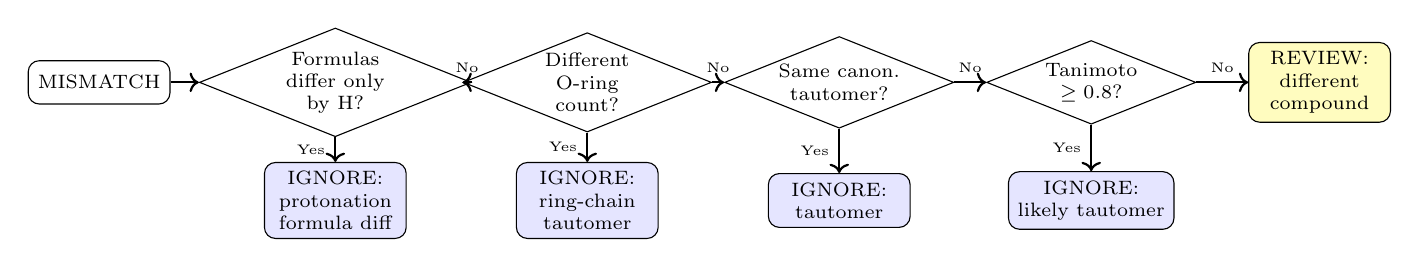
\begin{tikzpicture}[
  every node/.style={font=\scriptsize},
  box/.style={rectangle, draw, rounded corners, minimum width=1.8cm,
              minimum height=0.55cm, align=center},
  decision/.style={diamond, draw, aspect=2.5, inner sep=1pt,
                   align=center, font=\scriptsize},
  ignore/.style={box, fill=blue!10},
  review/.style={box, fill=yellow!25},
]
  \node[box] (input) at (0,0) {MISMATCH};
  \node[decision] (formula) at (3,0) {Formulas\\differ only\\by H?};
  \node[ignore] (protf) at (3,-1.5) {IGNORE:\\protonation\\formula diff};

  \node[decision] (ring) at (6.2,0) {Different\\O-ring\\count?};
  \node[ignore] (rct) at (6.2,-1.5) {IGNORE:\\ring-chain\\tautomer};

  \node[decision] (taut) at (9.4,0) {Same canon.\\tautomer?};
  \node[ignore] (keto) at (9.4,-1.5) {IGNORE:\\tautomer};

  \node[decision] (sim) at (12.6,0) {Tanimoto\\$\geq 0.8$?};
  \node[ignore] (likely) at (12.6,-1.5) {IGNORE:\\likely tautomer};

  \node[review] (diff) at (15.5,0) {REVIEW:\\different\\compound};

  \draw[->,thick] (input) -- (formula);
  \draw[->,thick] (formula) -- node[left,font=\tiny]{Yes} (protf);
  \draw[->,thick] (formula) -- node[above,font=\tiny]{No} (ring);
  \draw[->,thick] (ring) -- node[left,font=\tiny]{Yes} (rct);
  \draw[->,thick] (ring) -- node[above,font=\tiny]{No} (taut);
  \draw[->,thick] (taut) -- node[left,font=\tiny]{Yes} (keto);
  \draw[->,thick] (taut) -- node[above,font=\tiny]{No} (sim);
  \draw[->,thick] (sim) -- node[left,font=\tiny]{Yes} (likely);
  \draw[->,thick] (sim) -- node[above,font=\tiny]{No} (diff);
\end{tikzpicture}%
}
\end{center}

\smallskip
\footnotesize
\textbf{IGNORE}: the stored ModelSEED structure represents a different
tautomeric form than PubChem's canonical representation. No correction needed.\\
\textbf{REVIEW}: same molecular formula but low structural similarity ---
may indicate an incorrect cross-reference mapping to a positional or constitutional isomer.

\end{frame}

% =====================================================================
% PART 3: RESULTS
% =====================================================================

\begin{frame}{Validation Results}

\begin{columns}[T]
\begin{column}{0.45\textwidth}
\begin{table}[h]
\centering
\begin{tabular}{lrr}
\toprule
\textbf{Category} & \textbf{Count} & \textbf{\%} \\
\midrule
MATCH              & 19,984 & 65.9 \\
PROTONATION\_DIFF  &  4,365 & 14.4 \\
XREF\_CONFLICT     &  2,919 &  9.6 \\
MISMATCH           &  1,331 &  4.4 \\
NOT\_FOUND         &    832 &  2.7 \\
STEREO\_DIFF       &    683 &  2.3 \\
AMBIGUOUS          &    152 &  0.5 \\
Other              &     55 &  0.2 \\
\midrule
\textbf{Total}     & \textbf{30,321} & \textbf{100} \\
\bottomrule
\end{tabular}
\end{table}
\end{column}

\begin{column}{0.50\textwidth}
\textbf{Interpretation:}\small
\begin{itemize}\setlength\itemsep{2pt}
  \item \textbf{80.3\%} (MATCH + PROT\_DIFF) share the same
        connectivity and stereochemistry with PubChem
  \item \textbf{9.6\%} XREF\_CONFLICT --- ChEBI and KEGG
        cross-references point to different PubChem CIDs
  \item \textbf{4.4\%} MISMATCH --- different molecular
        connectivity; flagged for manual review
  \item \textbf{2.3\%} STEREO\_DIFF --- same connectivity,
        different stereochemistry assignments
  \item \textbf{2.7\%} NOT\_FOUND --- no matching PubChem
        record identified
  \item \textbf{0.5\%} AMBIGUOUS --- compound names resolve to
        multiple distinct PubChem CIDs
\end{itemize}
\end{column}
\end{columns}

\end{frame}

% =====================================================================
\begin{frame}{Lookup Strategy Breakdown}

\begin{columns}[T]
\begin{column}{0.45\textwidth}
\begin{table}[h]
\centering
\begin{tabular}{lr}
\toprule
\textbf{Strategy} & \textbf{Count} \\
\midrule
KEGG xref          &  9,717 \\
Name lookup        &  8,981 \\
ChEBI xref         &  6,245 \\
Xref conflict      &  2,919 \\
InChIKey recovery  &  2,228 \\
Ambiguous          &    152 \\
Xref resolved      &     79 \\
\midrule
\textbf{Total}     & \textbf{30,321} \\
\bottomrule
\end{tabular}
\end{table}
\end{column}

\begin{column}{0.50\textwidth}
\textbf{Agreement rate by strategy} (MATCH + PROT\_DIFF):
\begin{table}[h]
\centering
\footnotesize
\begin{tabular}{lrr}
\toprule
\textbf{Strategy} & \textbf{Agree} & \textbf{Rate} \\
\midrule
InChIKey recovery & 2,161 / 2,228  & 97.0\% \\
ChEBI xref        & 5,924 / 6,245  & 94.9\% \\
Name lookup       & 7,411 / 8,149  & 90.9\% \\
KEGG xref         & 8,775 / 9,717  & 90.3\% \\
Xref resolved     &    78 / 79     & 98.7\% \\
\bottomrule
\end{tabular}
\end{table}

\bigskip
\footnotesize
InChIKey recovery (Phase~2.5) yields the highest match rate at 97\%.
Among initial lookup strategies, ChEBI xrefs have the highest
agreement rate (94.9\%). KEGG xrefs produce the most protonation differences.
\end{column}
\end{columns}

\end{frame}

% =====================================================================
\begin{frame}{InChIKey Recovery: Phase 2.5 Impact}

\textbf{Phase 2.5 re-queries PubChem using the stored InChIKey} for
compounds that were NOT\_FOUND, MISMATCH, or STEREO\_DIFF after
Phases 1--2. This recovers cases where the stored structure is correct
but the cross-reference or name mapping was wrong.

\bigskip

\begin{columns}[T]
\begin{column}{0.45\textwidth}
\begin{table}[h]
\centering
\begin{tabular}{lr}
\toprule
\textbf{Result} & \textbf{Count} \\
\midrule
MATCH              & 2,161 (97.0\%) \\
STEREO\_DIFF       &    51 (2.3\%) \\
MISMATCH           &     2 (0.1\%) \\
Unknown            &    14 (0.6\%) \\
\midrule
\textbf{Total}     & \textbf{2,228} \\
\bottomrule
\end{tabular}
\end{table}
\end{column}

\begin{column}{0.50\textwidth}
\textbf{Interpretation:}\\[4pt]
\small
2,228 compounds that were previously unresolved or mismatched
were recovered, of which 97\% returned exact InChIKey matches.

\medskip
This indicates that for these compounds, the initial
discrepancies were due to incorrect cross-reference mappings
or name ambiguity rather than incorrect stored structures.

\medskip
\textbf{Without Phase~2.5}: these compounds would remain
classified as NOT\_FOUND or MISMATCH.
\end{column}
\end{columns}

\end{frame}

% =====================================================================
\begin{frame}{Correction Pipeline Outcomes}

\textbf{Automated corrections applied only to STEREO\_DIFF compounds.}
MISMATCH compounds classified for manual review (never auto-corrected).

\smallskip
\begin{table}[h]
\centering
\footnotesize
\begin{tabular}{lrrrl}
\toprule
\textbf{Category} & \textbf{Total} & \textbf{Corrected} & \textbf{Rejected} & \textbf{Action} \\
\midrule
STEREO\_DIFF       &    683 & 188 &  495 & Auto: PubChem $\geq$ stored stereo + pH~7 \\
PH7 normalization  & 30,321 &  13 &    1 & Phase 4: OpenBabel pH~7 \\
MISMATCH           &  1,331 &   0 & 1,331 & Classified for manual review \\
PROTONATION\_DIFF  &  4,365 &   0 &    0 & Skipped (pH-dependent) \\
XREF\_CONFLICT     &  2,919 &   0 &    0 & Unresolved (ChEBI $\neq$ KEGG) \\
AMBIGUOUS          &    152 &   0 &    0 & Skipped (names disagree) \\
NOT\_FOUND         &    832 &   0 &    0 & No PubChem reference \\
\bottomrule
\end{tabular}
\end{table}

\smallskip
\footnotesize
\textbf{Total corrections applied: 201 compounds}
(188 stereochemistry + 13 pH~7 protonation).\\[2pt]
\textbf{STEREO\_DIFF corrections} (188): each is pH~7-normalized (Phase~3.5)
before application so PubChem's neutral protonation does not overwrite
the curated ionization state.
\textbf{Rejections} (495): fewer stereocenters or inversions.\\[2pt]
\textbf{PH7} (Phase~4): deprotonates phosphate/sulfate groups;
free (non-ester) phosphates excluded ($\text{p}K_{\text{a}4} > 7$).

\end{frame}

% =====================================================================
\begin{frame}{\textcolor{acceptgreen}{STEREO\_DIFF Accepted}: PubChem Adds Missing Stereo}

\begin{columns}[T]
\begin{column}{0.48\textwidth}
\begin{center}
\textbf{cpd02877 --- Glycodeoxycholate}\\[3pt]

\includegraphics[width=\textwidth]{stereo_accepted_cpd02877.png}
\end{center}
\scriptsize
\textbf{cpd02877} (Glycodeoxycholate, name lookup).
PubChem defines all stereocenters for the bile acid scaffold.
\textcolor{acceptgreen}{Accepted} --- no existing stereocenters inverted.
\end{column}
\begin{column}{0.48\textwidth}
\begin{center}
\textbf{cpd04236 --- Cefotetan}\\[3pt]

\includegraphics[width=\textwidth]{stereo_accepted_cpd04236.png}
\end{center}
\scriptsize
\textbf{cpd04236} (Cefotetan, KEGG xref).
PubChem defines additional stereocenters on the cephalosporin ring.
\textcolor{acceptgreen}{Accepted} --- adds missing stereochemistry.
\end{column}
\end{columns}

\end{frame}

% =====================================================================
\begin{frame}{\textcolor{acceptgreen}{STEREO\_DIFF Accepted}: More Examples}

\begin{columns}[T]
\begin{column}{0.48\textwidth}
\begin{center}
\textbf{cpd03042 --- Porphyrin}\\[3pt]

\includegraphics[width=\textwidth]{stereo_accepted_cpd03042.png}
\end{center}
\scriptsize
\textbf{cpd03042} (Porphyrin, KEGG xref).
PubChem replaces the \texttt{UHFFFAOYSA} achiral placeholder with
a defined stereo block.
\textcolor{acceptgreen}{Accepted}.
\end{column}
\begin{column}{0.48\textwidth}
\begin{center}
\textbf{cpd05038 --- Rifapentine}\\[3pt]

\includegraphics[width=\textwidth]{stereo_accepted_cpd05038.png}
\end{center}
\scriptsize
\textbf{cpd05038} (Rifapentine, KEGG xref).
Macrolide antibiotic; PubChem record defines additional stereocenters.
\textcolor{acceptgreen}{Accepted}.
\end{column}
\end{columns}

\end{frame}

% =====================================================================
\begin{frame}{MISMATCH Examples: Tautomers and Wrong Mappings}

\begin{columns}[T]
\begin{column}{0.32\textwidth}
\begin{center}
\textbf{cpd00088 --- DCIP}\\[3pt]

\includegraphics[width=\textwidth]{mismatch_rejected_cpd00088.png}
\end{center}
\scriptsize
\textbf{cpd00088} (Dichloroindophenol, KEGG:C00102).\\
KEGG xref maps to a structurally different compound in PubChem.
\textcolor{rejectred}{REVIEW:different\_compound}.
\end{column}
\begin{column}{0.32\textwidth}
\begin{center}
\textbf{cpd00271 --- Ferricyanide}\\[3pt]

\includegraphics[width=\textwidth]{mismatch_rejected_cpd00271.png}
\end{center}
\scriptsize
\textbf{cpd00271} (Ferricyanide, KEGG:C00324).\\
PubChem record has different connectivity.
\textcolor{rejectred}{Rejected} --- requires manual review.
\end{column}
\begin{column}{0.32\textwidth}
\begin{center}
\textbf{cpd00532 --- Superoxide}\\[3pt]

\includegraphics[width=\textwidth]{mismatch_rejected_cpd00532.png}
\end{center}
\scriptsize
\textbf{cpd00532} (Superoxide, ChEBI:18421).\\
Molecular formula differs between stored and PubChem structures.
\textcolor{rejectred}{Rejected}.
\end{column}
\end{columns}

\smallskip
\scriptsize
All MISMATCH compounds are classified for manual review.
None are auto-corrected.

\end{frame}

% =====================================================================
\begin{frame}{MISMATCH Examples: More Cases}

\begin{columns}[T]
\begin{column}{0.32\textwidth}
\begin{center}
\textbf{cpd00166 --- B12}\\[3pt]

\includegraphics[width=\textwidth]{mismatch_rejected_cpd00166.png}
\end{center}
\scriptsize
\textbf{cpd00166} (Adenosylcobamide, KEGG:C00194).\\
Cobalt-containing cofactor; stored and PubChem structures differ.
\textcolor{rejectred}{Rejected} --- requires manual review.
\end{column}
\begin{column}{0.32\textwidth}
\begin{center}
\textbf{cpd00649 --- Coenzyme F420}\\[3pt]

\includegraphics[width=\textwidth]{mismatch_rejected_cpd00649.png}
\end{center}
\scriptsize
\textbf{cpd00649} (Coenzyme F420, KEGG:C00876).\\
Methanogenic cofactor; PubChem record has different connectivity.
\textcolor{rejectred}{Rejected}.
\end{column}
\begin{column}{0.32\textwidth}
\begin{center}
\textbf{cpd00792 --- Reduced F420}\\[3pt]

\includegraphics[width=\textwidth]{mismatch_rejected_cpd00792.png}
\end{center}
\scriptsize
\textbf{cpd00792} (Reduced F420, KEGG:C01080).\\
Reduced form of F420; same connectivity discrepancy as cpd00649.
\textcolor{rejectred}{Rejected}.
\end{column}
\end{columns}

\end{frame}

% =====================================================================
\begin{frame}{pH~7 Normalization: Phase 4 Examples}

\textbf{Phase 4} normalizes compounds to their pH~7 microspecies using
OpenBabel's \texttt{CorrectForPH(7.0)}. Only protonation-only changes
are accepted (same connectivity). Free (non-ester) phosphate
over-deprotonation is rejected ($\text{p}K_{\text{a}4} \approx 9.4 > 7$).

\medskip
\begin{table}[h]
\centering
\footnotesize
\begin{tabular}{llrrl}
\toprule
\textbf{Compound} & \textbf{Name} & \textbf{Old Chg} & \textbf{New Chg} & \textbf{Change} \\
\midrule
cpd00002 & ATP              & $-3$ & $-4$ & Deprotonated phosphate \\
cpd00008 & ADP              & $-2$ & $-3$ & Deprotonated phosphate \\
cpd00014 & UDP              & $-2$ & $-3$ & Deprotonated phosphate \\
cpd00031 & GDP              & $-2$ & $-3$ & Deprotonated phosphate \\
cpd00038 & GTP              & $-3$ & $-4$ & Deprotonated phosphate \\
cpd00081 & Sulfite          & $-1$ & $-2$ & Deprotonated sulfite \\
\midrule
\multicolumn{5}{l}{\textit{Rejected:}} \\
cpd00012 & Diphosphate (PPi) & $-3$ & --- & Free phosphate $\text{p}K_{\text{a}4}{=}9.4$ \\
\bottomrule
\end{tabular}
\end{table}

\smallskip
\footnotesize
13 corrections are single-proton deprotonations of ester-linked phosphate or
sulfate groups ($\text{p}K_\text{a} \approx 6.5$).
Free PPi (cpd00012) rejected: $\text{p}K_{\text{a}4}{=}9.4$, proton remains at pH~7.
Connectivity (InChIKey Block~1) unchanged in every case.

\end{frame}

% =====================================================================
\begin{frame}{Key Findings and Next Steps}

\textbf{Key findings:}\small
\begin{itemize}\setlength\itemsep{0pt}
  \item \textbf{80.3\%} (MATCH + PROT\_DIFF) share the same
        connectivity and stereochemistry with PubChem
  \item \textbf{Phase~2.5 recovered 2,228 compounds} (97\% match rate) ---
        initial discrepancies traced to incorrect mappings
  \item \textbf{188 stereo corrections applied} --- PubChem adds missing
        stereochemistry
  \item \textbf{13 pH~7 normalizations} --- deprotonation of phosphate/sulfate
        (free PPi excluded, $\text{p}K_{\text{a}4}{=}9.4$)
  \item \textbf{1,331 MISMATCH classified} --- for manual review
  \item \textbf{2,919 xref conflicts} remain unresolved (ChEBI $\neq$ KEGG)
\end{itemize}

\smallskip
\textbf{Next steps:}\small
\begin{enumerate}\setlength\itemsep{0pt}
  \item Resolve remaining XREF\_CONFLICT compounds (2,919)
  \item Manual review of MISMATCH compounds (1,331)
  \item Manual review of AMBIGUOUS compounds (152)
  \item Investigate NOT\_FOUND compounds (832) for missing xrefs
  \item Run full Phase~4 pH~7 normalization on complete dataset
\end{enumerate}

\end{frame}

% =====================================================================
% APPENDIX
% =====================================================================

\appendix
\begin{frame}
\centering
\vfill
{\Large \textbf{Appendix}}\\[6pt]
{\normalsize Detailed Category Analysis \& Technical Details}
\vfill
\end{frame}

% =====================================================================
\begin{frame}{Data Quality by Compound ID Range}

\begin{table}[h]
\centering
\footnotesize
\begin{tabular}{lrrrrrrrr}
\toprule
\textbf{ID Range} & \textbf{N} & \textbf{Match} & \textbf{Prot.} & \textbf{Mis.} & \textbf{Stereo} & \textbf{N/F} & \textbf{Amb.} & \textbf{Xref} \\
\midrule
0--9{,}999    & 9,463 & 49.1\% & 21.9\% & 3.9\% & 2.6\% & 0.0\% & 0.0\% & 22.1\% \\
10k--19{,}999 & 4,166 & 65.4\% & 15.7\% & 4.6\% & 2.3\% & 0.2\% & 0.0\% & 11.5\% \\
20k--29{,}999 & 5,773 & 76.2\% & 11.7\% & 3.3\% & 2.7\% & 0.6\% & 1.1\% &  4.2\% \\
30k--39{,}999 & 6,814 & 80.2\% &  9.1\% & 6.2\% & 1.5\% & 0.4\% & 1.1\% &  1.5\% \\
40k+          & 4,105 & 66.8\% &  8.5\% & 3.7\% & 2.1\% & 18.4\% & 0.4\% & 0.0\% \\
\bottomrule
\end{tabular}
\end{table}

\bigskip
\begin{itemize}
  \item Core metabolites (0--9{,}999) have high xref conflict rate (22.1\%)
        and protonation diffs (21.9\%) --- heavily cross-referenced
  \item Compounds $>$40{,}000 have 18.4\% NOT\_FOUND --- recently added with
        sparse external references
  \item Match rate improves in mid-ranges (20k--40k) --- 76--80\%
  \item MISMATCH rate peaks in 30k--40k range (6.2\%)
\end{itemize}

\end{frame}

% =====================================================================
\begin{frame}{Mismatch Analysis}

\begin{columns}[T]
\begin{column}{0.48\textwidth}
\textbf{By lookup strategy:}
\begin{table}[h]
\centering
\begin{tabular}{lr}
\toprule
\textbf{Strategy} & \textbf{Mismatches} \\
\midrule
KEGG xref       &   600 (45.1\%) \\
Name lookup     &   523 (39.3\%) \\
ChEBI xref      &   206 (15.5\%) \\
InChIKey lookup &     2 (0.2\%) \\
\midrule
\textbf{Total} & \textbf{1,331} \\
\bottomrule
\end{tabular}
\end{table}

\bigskip
\footnotesize
KEGG xrefs account for 45.1\% of all mismatches, followed by
name lookups (39.3\%). ChEBI xrefs produce the fewest mismatches (15.5\%).
InChIKey recovery yields only 2 mismatches out of 2,228 lookups.
\end{column}

\begin{column}{0.48\textwidth}
\textbf{Stereo diffs by strategy:}
\begin{table}[h]
\centering
\begin{tabular}{lr}
\toprule
\textbf{Strategy} & \textbf{Count} \\
\midrule
KEGG xref       & 315 (46.1\%) \\
Name lookup     & 215 (31.5\%) \\
ChEBI xref      & 102 (14.9\%) \\
InChIKey lookup &  51 (7.5\%) \\
\midrule
\textbf{Total} & \textbf{683} \\
\bottomrule
\end{tabular}
\end{table}

\bigskip
\footnotesize
KEGG xrefs are the largest source of stereo differences (46.1\%).
188 of 683 STEREO\_DIFF compounds passed validation and were corrected (27.5\%).
\end{column}
\end{columns}

\end{frame}

% =====================================================================
\begin{frame}{Protonation Difference Analysis}

\begin{columns}[T]
\begin{column}{0.45\textwidth}
\textbf{By lookup strategy:}
\begin{table}[h]
\centering
\begin{tabular}{lrr}
\toprule
\textbf{Strategy} & \textbf{Count} & \textbf{Rate} \\
\midrule
KEGG xref    & 2,880 & 29.6\% \\
Name lookup  & 1,324 & 16.3\% \\
ChEBI xref   &   144 &  2.3\% \\
Xref resolved &   17 & 21.5\% \\
\midrule
\textbf{Total} & \textbf{4,365} & \\
\bottomrule
\end{tabular}
\end{table}
\end{column}

\begin{column}{0.50\textwidth}
\textbf{Interpretation:}\small
\begin{itemize}\setlength\itemsep{3pt}
  \item KEGG produces $20\times$ more protonation diffs than ChEBI
  \item ModelSEED stores pH~7 charge states;
        PubChem stores neutral forms
  \item \textbf{Not auto-corrected}: the difference reflects
        different pH conventions, not an error
  \item Phase~4 pH~7 normalization addresses compounds where
        ModelSEED's stored protonation was inconsistent with pH~7
\end{itemize}
\end{column}
\end{columns}

\bigskip
\begin{center}
\footnotesize
\begin{tabular}{llll}
\textbf{Example} & \textbf{Compound} & \textbf{ModelSEED} & \textbf{PubChem} \\
cpd00002 & ATP & ATP$^{3-}$ (partially protonated) & ATP$^{4-}$ (fully deprotonated) \\
cpd00012 & Diphosphate & PP$_\text{i}^{3-}$ (one P-OH) & PP$_\text{i}^{4-}$ (fully ionized) \\
\end{tabular}
\end{center}

\end{frame}

% =====================================================================
\begin{frame}{PROTONATION\_DIFF Examples}

\begin{columns}[T]
\begin{column}{0.48\textwidth}
\begin{center}
\textbf{cpd00043 --- UDP-Galactose}\\[3pt]

\includegraphics[width=\textwidth]{prot_rejected_cpd00043.png}
\end{center}
\scriptsize
ModelSEED stores the pH~7 protonation state.
PubChem stores a different protonation state.
\textcolor{warnblue}{Skipped} --- same compound at different pH.
\end{column}
\begin{column}{0.48\textwidth}
\begin{center}
\textbf{cpd00074 --- Selenocysteine}\\[3pt]

\includegraphics[width=\textwidth]{prot_rejected_cpd00074.png}
\end{center}
\scriptsize
Different protonation state: ModelSEED stores the
pH~7 form, PubChem stores the neutral form.
\textcolor{warnblue}{Skipped}.
\end{column}
\end{columns}

\smallskip
\footnotesize
\textit{Not auto-corrected: the protonation difference reflects the
intended pH~7 representation in ModelSEED vs.\ the neutral form in PubChem.}

\end{frame}

% =====================================================================
\begin{frame}{XRef Conflict Analysis}
\small
\textbf{2,919 compounds} have conflicting ChEBI and KEGG cross-references
pointing to different PubChem CIDs. Only 79 resolved by Phase~1.5/1.7.

\vspace{-2pt}
\begin{columns}[T]
\begin{column}{0.48\textwidth}
\textbf{Resolution strategy:}\footnotesize
\begin{itemize}\setlength\itemsep{0pt}
  \item Compare candidate InChIKeys to stored InChIKey
  \item Priority: exact match $>$ blocks~1+2 $>$ block~1
  \item Source preference: ChEBI $>$ KEGG
  \item Phase~1.7: fetch full CID properties for remaining
\end{itemize}

\textbf{Why so many unresolved?}\footnotesize
\begin{itemize}\setlength\itemsep{0pt}
  \item Core metabolites (0--9k) most affected (22.1\%)
  \item Many xrefs map to different protonation forms
  \item Neither candidate matches stored InChIKey exactly
\end{itemize}
\end{column}

\begin{column}{0.48\textwidth}
\textbf{Example} (cpd00059):\footnotesize\\[2pt]
ChEBI $\to$ CID~54679076 \quad vs \quad KEGG C00072 $\to$ CID~54670067

\smallskip
\footnotesize
Both CIDs correspond to PubChem records for the same compound
but with different charge states or stereoisomers.
Requires manual review to determine which is correct.

\smallskip
\textbf{Impact}: 2,919 compounds cannot be validated
until conflicts are resolved. Concentrated in the 0--10k
ID range where compounds have the most cross-references.
\end{column}
\end{columns}

\end{frame}

% =====================================================================
\begin{frame}{Safety Features and Validation Checks}
\small
\begin{columns}[T]
\begin{column}{0.48\textwidth}
\textbf{Quality Gates}\footnotesize
\begin{itemize}\setlength\itemsep{0pt}
  \item Formula cross-check for MISMATCH
  \item Stereo center counting (RDKit) for STEREO\_DIFF
  \item InChI stereo layer comparison (no inversions)
  \item SMILES$\leftrightarrow$InChIKey consistency check
  \item ChEBI/KEGG xref cross-validation
  \item Multi-name ambiguity detection
  \item pH~7 connectivity check (no bond changes)
\end{itemize}

\smallskip
\textbf{Data Preservation}\footnotesize
\begin{itemize}\setlength\itemsep{0pt}
  \item Never overwrites original structures file
  \item Corrections log with ISO~8601 timestamps
  \item Formula/Charge recomputed from corrected InChI
  \item Atomic writes (temp file + rename)
\end{itemize}
\end{column}

\begin{column}{0.48\textwidth}
\textbf{Cache and Resumability}\footnotesize
\begin{itemize}\setlength\itemsep{0pt}
  \item SQLite cache (CIDs, InChIKeys, SMILES)
  \item \texttt{-{}-clear-cache} for fresh runs
  \item Rate-limited PubChem API (5~req/s)
  \item Thread-safe conflict tracking
\end{itemize}

\smallskip
\textbf{Output files}\scriptsize
\begin{itemize}\setlength\itemsep{0pt}
  \item \texttt{pubchem\_validation\_report.tsv}
  \item \texttt{pubchem\_mismatches.tsv}
  \item \texttt{pubchem\_stereo\_diffs.tsv}
  \item \texttt{pubchem\_protonation\_diffs.tsv}
  \item \texttt{pubchem\_corrections\_log.tsv}
  \item \texttt{pubchem\_rejected\_corrections.tsv}
  \item \texttt{pubchem\_protonation\_corrections.tsv}
  \item \texttt{pubchem\_review\_different\_compounds.tsv}
\end{itemize}
\end{column}
\end{columns}

\end{frame}

\end{document}
